% Figure 3 (optimized): data augmentation pipeline, redrawn as vector TikZ.
% Compiles with pdfLaTeX, XeLaTeX or LuaLaTeX (no Hebrew inside), so it can also be pasted
% straight into the paper as a tikzpicture. Natural width = 16cm (ACL \textwidth).
\documentclass[10pt,border=2pt]{standalone}
\usepackage{iftex}
\ifPDFTeX \usepackage{times} \else \usepackage{fontspec}\setmainfont{FreeSerif.otf}[BoldFont=FreeSerifBold.otf,ItalicFont=FreeSerifItalic.otf] \fi
\usepackage{tikz}
\usetikzlibrary{positioning,arrows.meta,fit,backgrounds,calc}
% Colour encodes the role of each step (legend at bottom); every box is also labelled, so greyscale print works
\definecolor{llm}{HTML}{CFE3F3}    % negative-augmentation processing step
\definecolor{filt}{HTML}{F6D3D3}   % filtering step
\definecolor{pos}{HTML}{D6EEDC}    % positive augmentation
\definecolor{data}{HTML}{EFEFEF}   % data / artefact
\begin{document}\hyphenpenalty=10000\exhyphenpenalty=10000
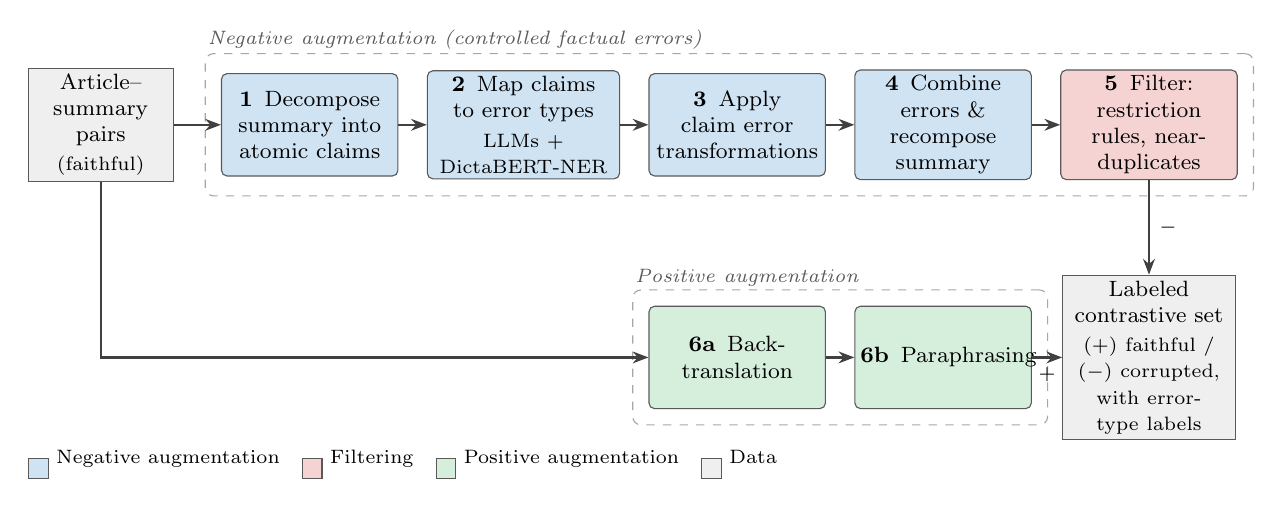
\begin{tikzpicture}[
  font=\footnotesize, node distance=4mm and 3.6mm, >={Stealth[length=2mm]},
  box/.style={draw=black!65, rounded corners=2pt, align=center, minimum height=13mm, text width=21mm, inner sep=2pt},
  dat/.style={box, fill=data, rounded corners=0pt},
  lane/.style={draw=black!35, dashed, rounded corners=3pt, inner sep=2mm},
  lanelabel/.style={font=\scriptsize\itshape, text=black!65, anchor=south west, inner sep=1pt},
  arr/.style={->, draw=black!75, thick}]

% ---- input + negative lane ----
\node[dat, text width=17mm] (in) {Article--\\summary pairs\\[1pt]\scriptsize(faithful)};
\node[box, fill=llm, right=6mm of in] (s1) {\textbf{1}\enspace Decompose summary into atomic claims};
\node[box, fill=llm, right=of s1, text width=23mm] (s2) {\textbf{2}\enspace Map claims to error types\\[1pt]\scriptsize LLMs + DictaBERT-NER};
\node[box, fill=llm, right=of s2] (s3) {\textbf{3}\enspace Apply claim error transformations};
\node[box, fill=llm, right=of s3] (s4) {\textbf{4}\enspace Combine errors \& recompose summary};
\node[box, fill=filt, right=of s4] (s5) {\textbf{5}\enspace Filter: restriction rules, near-duplicates};

% ---- output + positive lane (same row) ----
\node[dat, below=12mm of s5, text width=20.5mm] (out) {Labeled contrastive set\\[1pt]\scriptsize ($+$) faithful / ($-$) corrupted, with error-type labels};
\node[box, fill=pos] (p2) at (s4 |- out) {\textbf{6b}\enspace Paraphrasing};
\node[box, fill=pos] (p1) at (s3 |- out) {\textbf{6a}\enspace Back-\\translation};

\begin{scope}[on background layer]
  \node[lane, fit=(s1)(s2)(s5)] (negl) {};
  \node[lane, fit=(p1)(p2)] (posl) {};
\end{scope}
\node[lanelabel] at (negl.north west) {Negative augmentation (controlled factual errors)};
\node[lanelabel] at (posl.north west) {Positive augmentation};

% ---- arrows ----
\draw[arr] (in) -- (s1);
\foreach \a/\b in {s1/s2,s2/s3,s3/s4,s4/s5,p1/p2} \draw[arr] (\a) -- (\b);
\draw[arr] (s5) -- node[right, font=\scriptsize]{$-$} (out);
\draw[arr] (p2) -- node[below, font=\scriptsize]{$+$} (out);
\draw[arr] (in.south) |- (p1.west);

% ---- legend (one row, under the input column, clear of all nodes) ----
\newcommand{\sw}[1]{\tikz[baseline=-0.6ex]\node[fill=#1,draw=black!65,minimum size=2.5mm,inner sep=0]{};}
\node[anchor=north west, font=\scriptsize, inner sep=0] at ([yshift=-3mm]in.west |- posl.south)
  {\sw{llm}~Negative augmentation\quad \sw{filt}~Filtering\quad \sw{pos}~Positive augmentation\quad \sw{data}~Data};
\end{tikzpicture}
\end{document}
